%%%% ijcai09.tex

\typeout{IJCAI-09 Instructions for Authors}

% These are the instructions for authors for IJCAI-09.
% They are the same as the ones for IJCAI-07 with superficical wording
%   changes only.

\documentclass{article}
% The file ijcai09.sty is the style file for IJCAI-09 (same as ijcai07.sty).
\usepackage{ijcai09}
\usepackage{url}
\usepackage{graphicx}
\usepackage{listings}
\usepackage{subfigure}

% Use the postscript times font!
\usepackage{times}

% the following package is optional:
%\usepackage{latexsym} 

% Following comment is from ijcai97-submit.tex:
% The preparation of these files was supported by Schlumberger Palo Alto
% Research, AT\&T Bell Laboratories, and Morgan Kaufmann Publishers.
% Shirley Jowell, of Morgan Kaufmann Publishers, and Peter F.
% Patel-Schneider, of AT\&T Bell Laboratories collaborated on their
% preparation.

% These instructions can be modified and used in other conferences as long
% as credit to the authors and supporting agencies is retained, this notice
% is not changed, and further modification or reuse is not restricted.
% Neither Shirley Jowell nor Peter F. Patel-Schneider can be listed as
% contacts for providing assistance without their prior permission.

% To use for other conferences, change references to files and the
% conference appropriate and use other authors, contacts, publishers, and
% organizations.
% Also change the deadline and address for returning papers and the length and
% page charge instructions.
% Put where the files are available in the appropriate places.

\title{HTTP Redirect Attack}
\author{Robert Christensen, Phil Lundrigan, Mark Thueson\\
Department of Computer Science\\
University of Utah \\
robert.christensen@gmail.com, philiplundrigan@gmail.com, m\_thueson@hotmail.com}

\begin{document}

\maketitle

\begin{abstract}
  Your abstract should concisely answer the following three questions: 1) what problem are you addressing? 2) what approach are you taking to solve the problem? 3) what are your results?
  
  Place the abstract at the beginning of the first column 3$''$ from the
top of the page, unless that does not leave enough room for the title
and author information. Use a slightly smaller width than in the body
of the paper. Head the abstract with ``Abstract'' centered above the
body of the abstract in a 12-point bold font. The body of the abstract
should be in the same font as the body of the paper.

The abstract should be a concise, one-paragraph summary describing the
general thesis and conclusion of your paper. A reader should be able
to learn the purpose of the paper and the reason for its importance
from the abstract. The abstract should be no more than 200 words long.
\end{abstract}

\section{Introduction}
Many people when attempting to connect to a secure website, such as a banking website, simply enter the well-known web address such as www.chase.com. Users often assume the a connection will be established with the desired host.  If applicable, especially for banking sites, the user will assume the connection established between the web browser and server will be secured.  However, the web assumes unsecure connections such as http and will establish a secure https connection only when a special request is made.  When the well known web address www.chase.com is requested, the web server will request the IP address of the chase.com server over DNS.  When the correct IP server address is known to the client, the client will request the web page at http://www.chase.com.  In order to migrate the user to a secure, encrypted version of the website, a redirect message is returned from the server to point the client the secure website https://www.chase.com.  This inherent redirect is subject to a number of different attacks; however this work focuses on the possibility of intercepting the redirect packet and instead servicing the initial http request with a mock site.  We will show that an adversary can setup a public access point and perform such an attack.  If more time were given various solutions would also be explored that would mitigate the possibility of such attacks.


\section{Related Work}
There are many works that can be found about phishing schemes that perform similar attacks.  Most of these use techniques such as ARP cache or DNS cache poisoning to allow all network traffic to be routed through them, the most notable of these is \texttt{sslstrip}\cite{sslstrip}.  These tools however are mostly focused on changing the redirect message to contain a homograph-similar site name (such as www.cha5e.com etc.).

Other works discuss the correctness of even allowing an http redirect to point to an https citing security gaps such as the ones used by the aforementioned tools.

\section{Adversary Model}
This attack is demonstrated as a type of Man In The Middle attack.  An adversary can provide a public access point and allow anyone to connect to the internet via his connection.  Being the first hop in their connection all packets are available to sniff and alter as desired.  The adversary would use a filter to forward all normal traffic but would keep a listing of sites that it has doctored and replace all redirects to https versions of these sites with the doctored ones.  This would present the victim with a website that appears to be the normal https site they are used to but would actually only be a normal http site with the correct address that they initially typed (as opposed to a homograph-similar address).  Since many people are unaware of the difference between http and https the adversary would be able to acquire sensitive information from the victim such as usernames and passwords.

%%%%%%%%%% Figure %%%%%%%%%%
\begin{figure}[t]
\begin{center}

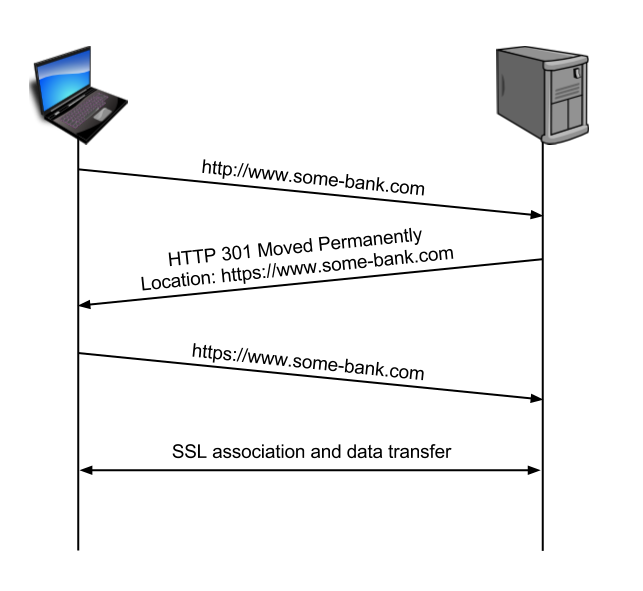
\includegraphics[width=2.3in]{normal_redirect.png} 
\caption{A typical HTTP redirect to switch from HTTP to HTTPS} 
\label{fg:redirect}

\end{center}
\end{figure}
%%%%%%%%%%%%%%%%%%%%%%%%

\section{Methodology}
We were unable to implement any solution to this problem but thought of a few ways one would go about implementing one.
One idea is to build a table into browsers that contains lists of sites that should always resolve using the https version instead of http.  This list could be maintained through browser updates and other methods but may end up causing too much upkeep overhead or become unsynchronized with the actual state of the internet.

Any site that uses one time passwords can easily be protected against these types of attacks.  If a client is attempting to connect via an untrusted access point they can be issued a one time password via a secondary trusted authority that is registered to their account such as a cell phone.  This prevents the client from ever entering in their long term password and an adversary from aquiring any sensitive information.  While this does provide additional security it also makes authenticating harder on the user.  It also makes the assumption that such a secondary authority is available.

Multiple stage authentication is an option that servers can provide to guard against these attacks as well.  To implement this the server would prompt the client for minimal information such as an account number or username.  The server can then issue challenges set by the client (such as personal questions) which allows the clien to to authenticate the server.  Only once these stages are complete would the server prompt for sensitive information such as a password.

Some people purpose the idea that the redirect message should be exchanged for an error message that prompts the user to manually contact the server via the https address.  This may thwart many problems similar to the one in this paper but also creates a less user friendly method.

Ideally there would be a way to make it the networks responsibility so it could be done without bothering either the client or the server.  In order for this to occur major changes to the current network would have to be made.  Implementing IPSec or transitioning to Content Centric Networking would actually solve all attacks of this nature.

%%%%%%%%%% Figure %%%%%%%%%%
\begin{figure}[t]
\begin{center}

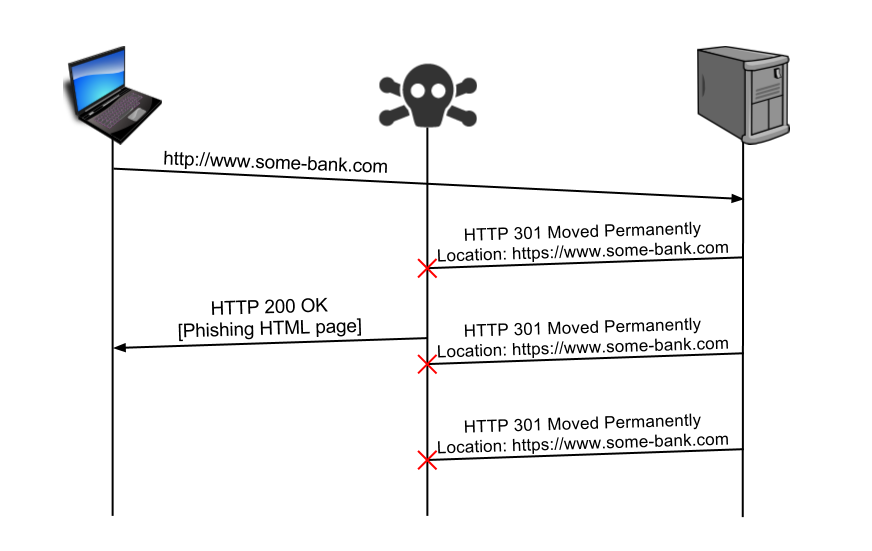
\includegraphics[width=3in]{redirect_attack.png} 
\caption{A HTTP Redirect attack} 
\label{fg:attack}

\end{center}
\end{figure}
%%%%%%%%%%%%%%%%%%%%%%%%

\section{Implementation / Experimentation}

\section{Conclusion}

\section{Temp}

reference to original idea\cite{offpath}

reference to \texttt{netfilter}\cite{netfilter} and \texttt{netfilter\_queue}\cite{netfilterQueue}

% Here is a reference to different bib formats:
%	http://en.wikibooks.org/wiki/LaTeX/Bibliography_Management
\bibliographystyle{plain}
\bibliography{ref}

\end{document}

